\chapter{Fluoride Salt Cooled High-Temperature Reactor Benchmark}
\label{chap:fhr-benchmark}
% Main Gist 
% - The work I did for the FHR Benchmark
% Structure 
% - Specifications of benchmark problem
% - Results from benchmark
% Appendix? 
% - More details about the geometry 

The \gls{FHR} is a reactor concept that uses \gls{TRISO}-based fuel and a 
low-pressure liquid fluoride-salt coolant.
\gls{FHR} technology combines FLiBE coolant from \gls{MSR} technology and 
\gls{TRISO} particles from \gls{VHTR} technology to enable a reactor with 
low operating pressure, large thermal margin, and accident-tolerant 
qualities.
To address the technical challenges of \gls{AHTR} modeling, such as multiple 
heterogeneity and material cross-section data, the \gls{OECD}-\gls{NEA} and 
\gls{Georgia Tech} initiated the \gls{FHR} benchmark for the \gls{AHTR} design 
in 2019 \cite{noauthor_fluoride_nodate}. 
The \gls{AHTR} is a type of \gls{FHR} that has plate-based fuel in a hexagonal 
fuel assembly. 
In section \ref{sec:fhr}, we gave an overview of the \gls{FHR} concept, 
a high-level description of the \gls{AHTR} design, a review of previous efforts 
towards modeling these designs, and how these efforts led to the 
initiation of the benchmark. 

The \gls{FHR} benchmark has several phases, starting with a single fuel assembly 
simulation without burnup and gradually extending to full core depletion. 
Table \ref{tab:phases} outlines the complete and incomplete benchmark phases.

\begin{table}[H]
    \centering
    \onehalfspacing
    \caption{Phases of the \gls{FHR} benchmark \cite{noauthor_fluoride_nodate}.}
	\label{tab:phases}
    \footnotesize
    \begin{tabular}{lclc}
    \hline 
    \textbf{Phases}& \textbf{Sub-phases} & \textbf{Description} & \textbf{Completed?} \\
    \hline
    \multirow{ 3}{5cm}{\textbf{Phase I: Fuel assembly (2D/3D with depletion)}} & I-A & 2D model, steady-state (no depletion) & \checkmark\\
    &I-B & 2D model depletion & \checkmark\\
    &I-C & 3D model depletion &\\
    \hline
    \multirow{2}{5cm}{\textbf{Phase II: 3D full core with depletion}}&II-A & Steady-state (no depletion) &\\
    &II-B & Depletion &\\
    \hline 
    \multirow{ 2}{5.5cm}{\textbf{Phase III: 3D full core with feedback \& multicycle analysis}}&III-A & Full core depletion with feedback &\\
    &III-B & Multicycle analysis &\\
    \hline
    \end{tabular}
\end{table}

In the subsequent sections, we will describe the benchmark's specifications for 
the \gls{AHTR} design and phase I. Then, we will share our phase I-A and I-B 
results. 

\section{Benchmark Specifications: AHTR Design}
The \gls{AHTR} has 3400 MWt thermal power and 1400 MW electric power 
\cite{varma_ahtr_2012}. 
Figure \ref{fig:reactor-schematic} shows the reactor schematic and a vertical 
cut of the reactor vessel. 
\begin{figure}[]
    \centering
    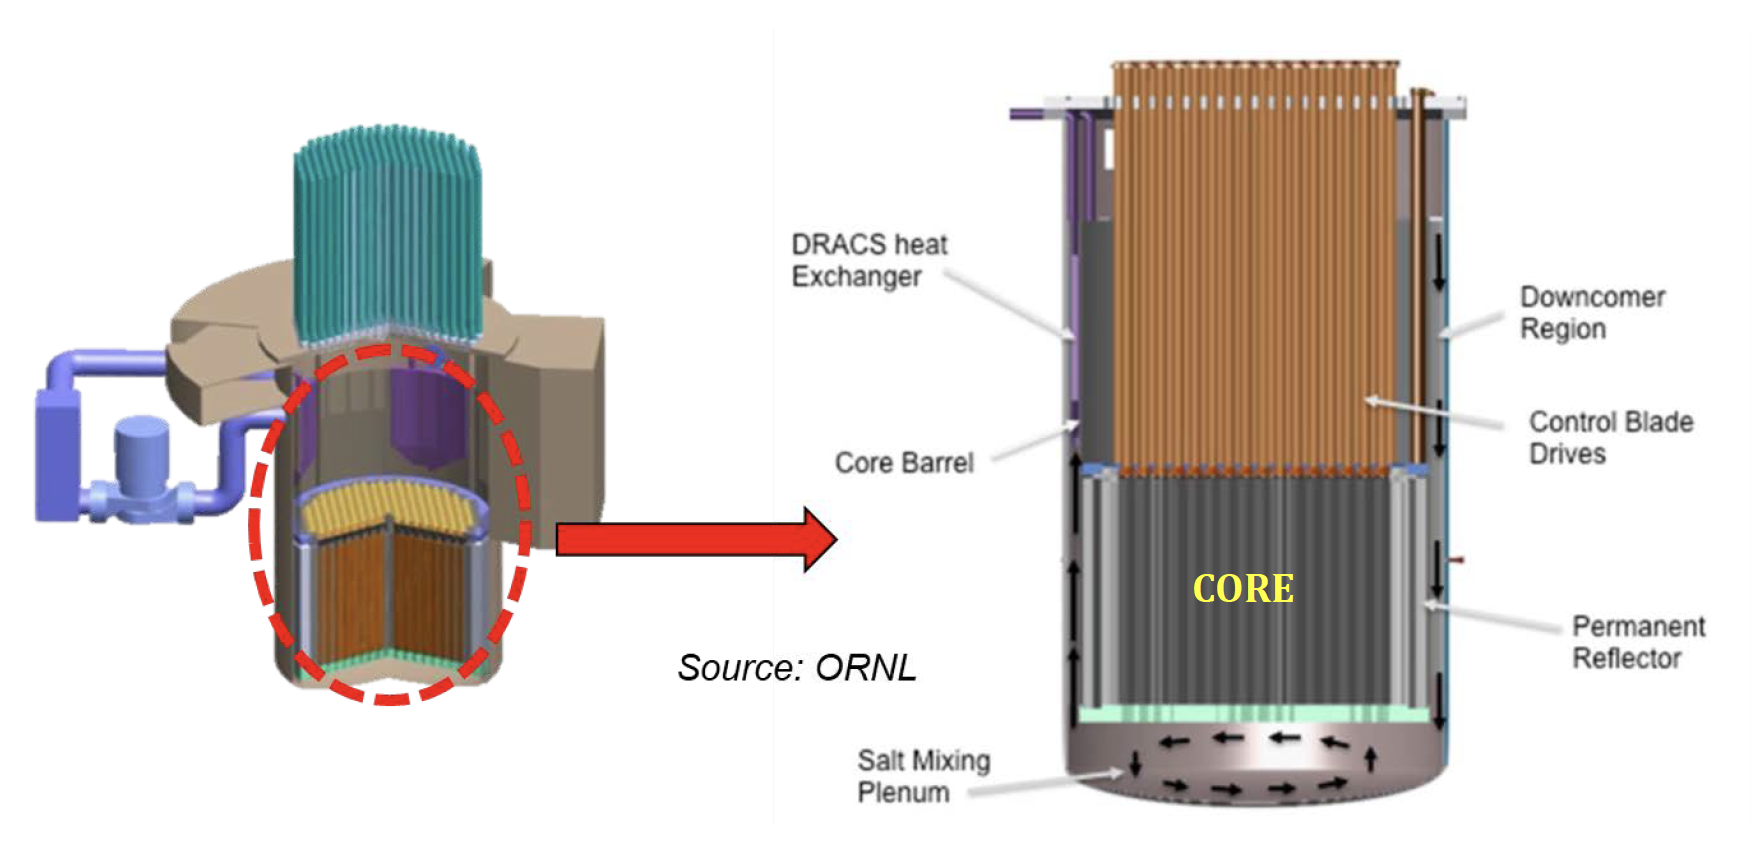
\includegraphics[width=0.9\linewidth]{reactor-schematic.png} 
    \caption{\acrlong{AHTR} schematic (left) and vessel (right) 
    \cite{noauthor_fluoride_nodate}.}
    \label{fig:reactor-schematic}
\end{figure}
Figure \ref{fig:ahtr} shows the geometry of a single fuel assembly and all 
assemblies' configuration in the core.
A detailed 2D view of the \gls{AHTR}'s hexagonal fuel assembly is shown in 
Figure \ref{fig:ahtr-fuel-assembly}.  
\begin{figure}[]
    \centering
    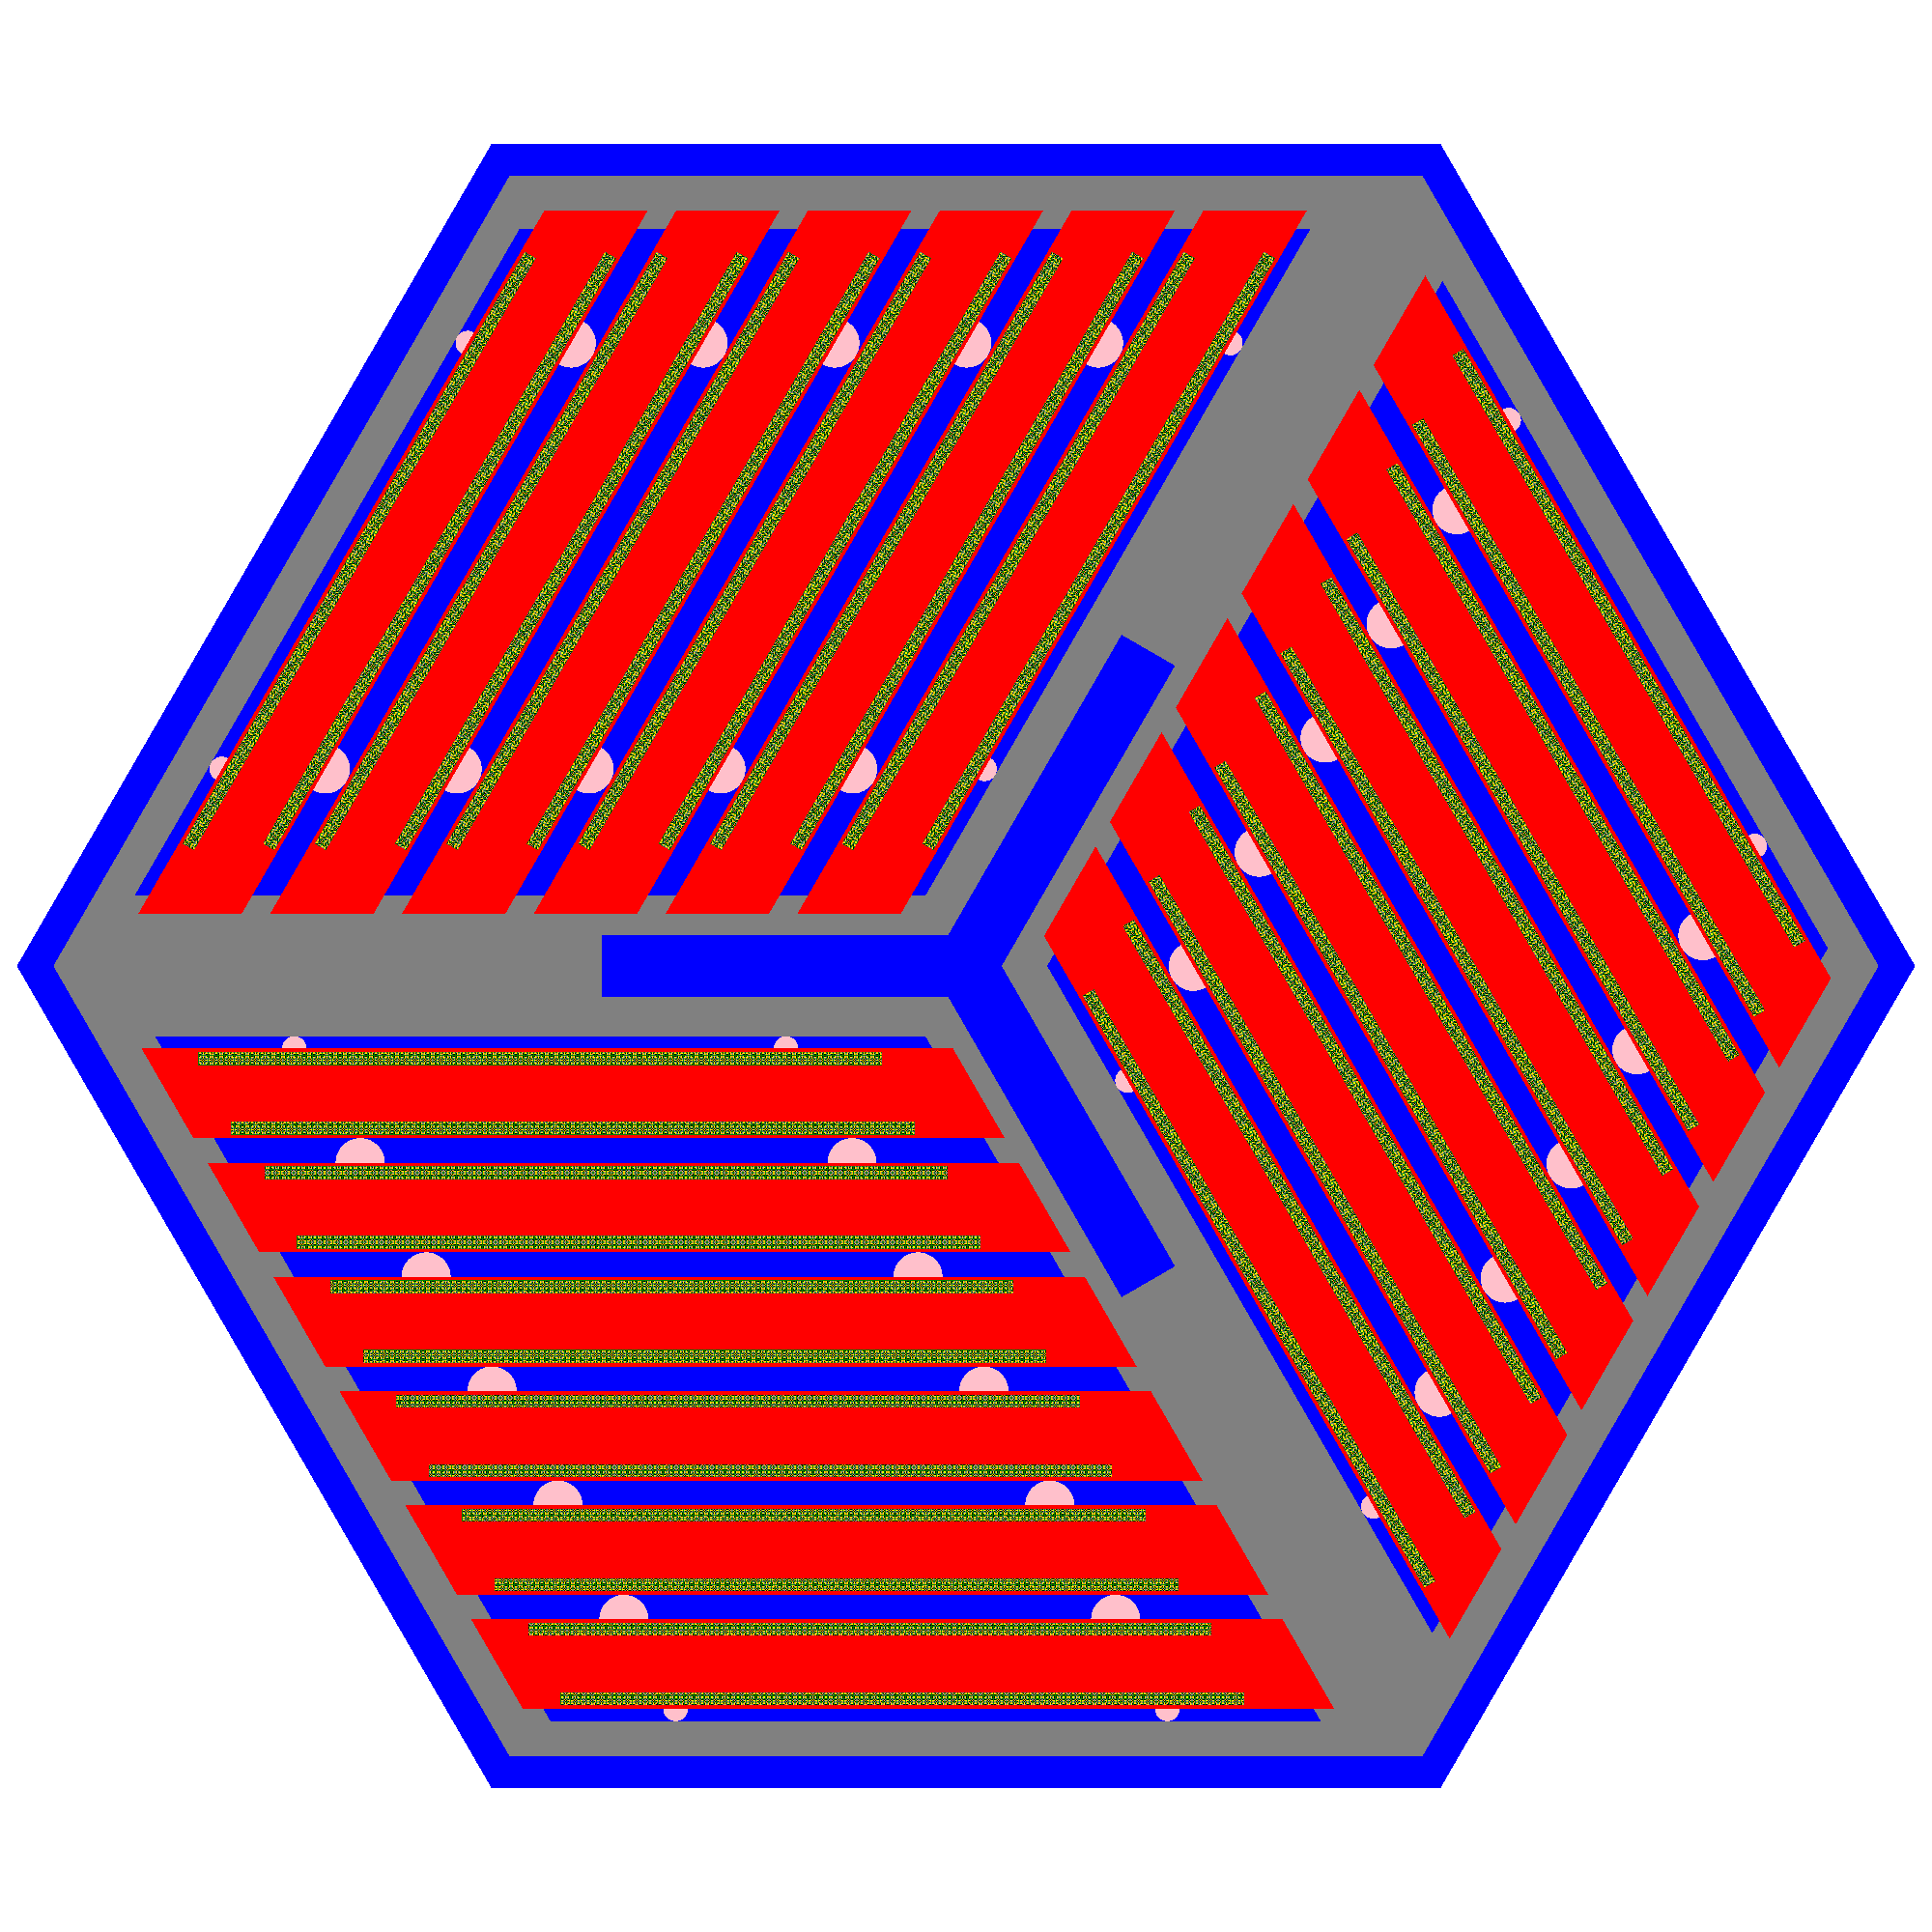
\includegraphics[width=0.5\linewidth]{ahtr-fuel-element.png} 
    \caption{\acrlong{AHTR} fuel assembly with 18 fuel plates arranged in 
    three diamond-shaped sectors, with a central Y-shaped and external channel 
    graphite structure. Blue: FliBE coolant in between fuel assemblies and plates, 
    and in the control rod slot, Gray: graphite structural components, 
    Red: graphite fuel plank, Pink: graphite spacers, Green: graphite matrix 
    with embedded TRISO particles.}
    \label{fig:ahtr-fuel-assembly}
\end{figure}
It features plate-type fuel with hexagonal fuel assembly consisting of eighteen 
planks arranged in three diamond-shaped sectors, with a central Y-shaped 
structure and external channel (wrapper).
The diamond-shaped sections have 120-deg rotational symmetry with each other 
\cite{varma_ahtr_2012,ramey_monte_2018,noauthor_fluoride_nodate}. 
The fuel planks have semi-cylindrical spacers attached, their radius being 
equal to the coolant channel thickness. 

The external channel wrapper and structural Y-shape, as seen in Figure 
\ref{fig:y-shape}, are made of C-C composite and have extra notches to hold 
the fuel plates in place.
\begin{figure}[]
    \centering
    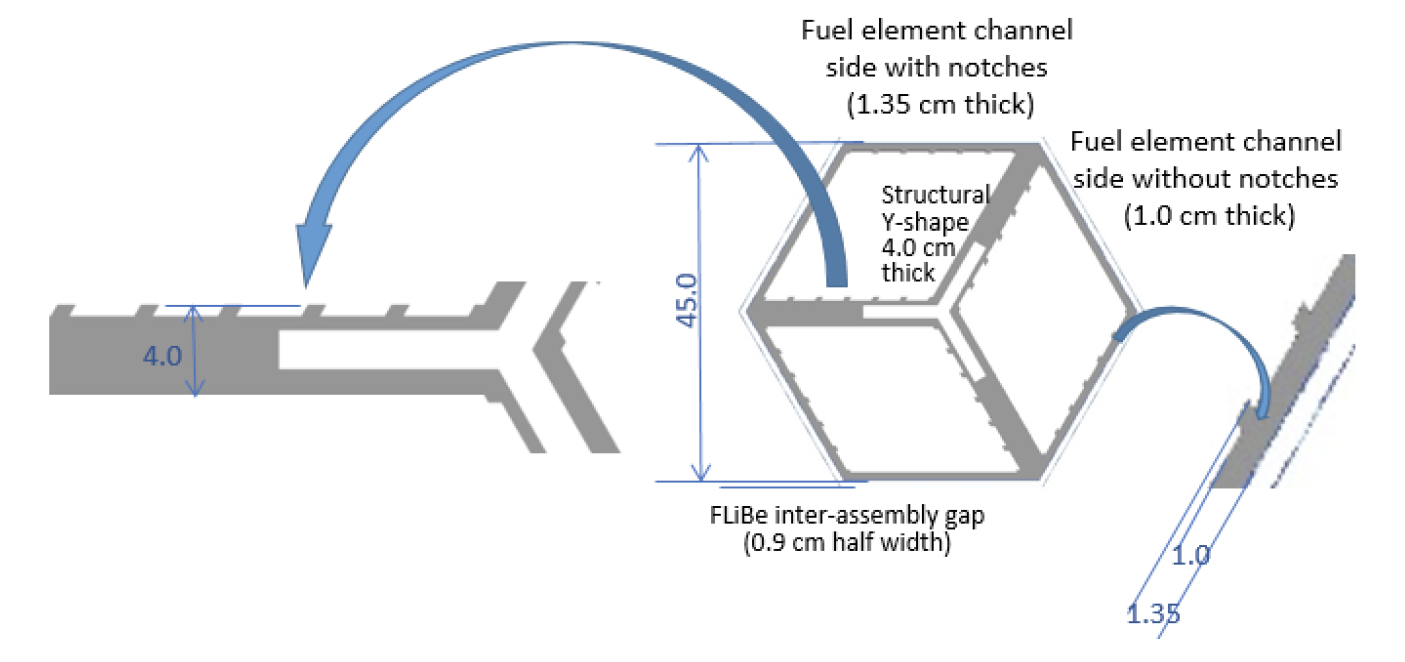
\includegraphics[width=0.8\linewidth]{y-shape.png} 
    \caption{\acrlong{AHTR} fuel assembly's structural components 
    \cite{noauthor_fluoride_nodate}.}
    \label{fig:y-shape}
\end{figure}
The gap between the fuel assemblies and fuel plates are filled with \gls{FLiBe}
coolant. 
The Y-shaped control rod slot at the center of the Y-shape structure contains 
\gls{FLiBe} coolant when the control blade is not in the slot
\cite{varma_ahtr_2012,ramey_monte_2018,noauthor_fluoride_nodate}.
Each fuel plank is made of an isostatically pressed carbon with fuel stripes 
on each outer side of the plank, as seen in Figure \ref{fig:ahtr-fuel-plank}. 
\begin{figure}[]
    \centering
    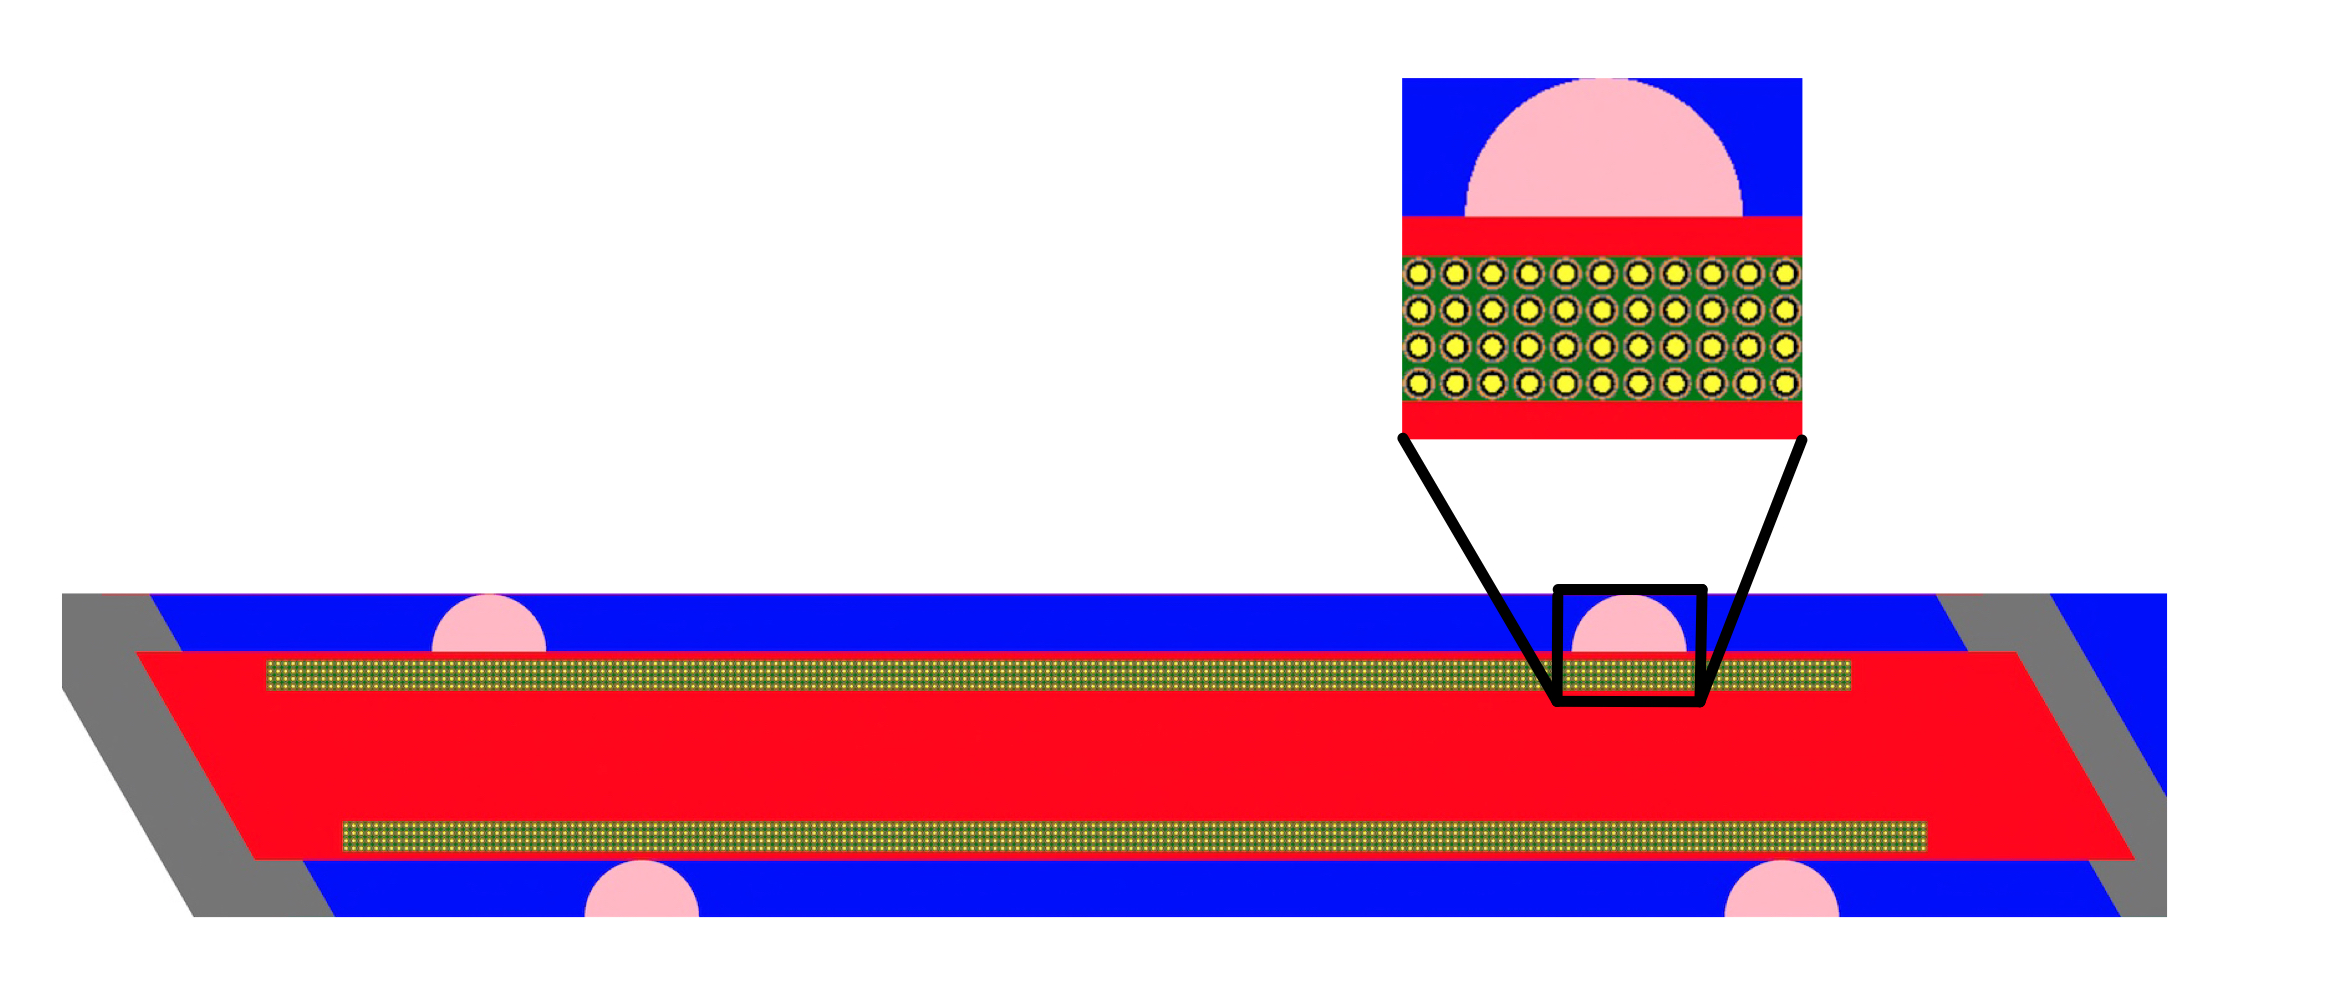
\includegraphics[width=0.75\linewidth]{ahtr-fuel-plank.png} 
    \caption{\acrlong{AHTR}'s fuel plank, with magnification of 
    a spacer and segment of the fuel stripe with embedded TRISO particles.}
    \label{fig:ahtr-fuel-plank}
\end{figure}
The fuel stripes are prismatic regions composed of a graphite matrix filled with 
a cubic lattice of \gls{TRISO} particles with a 40\% packing fraction. 
The lattice is 210 \gls{TRISO} particles wide in the x-direction, four particles 
deep in the y-direction, and 5936 particles tall in the z-direction. 
Each \gls{TRISO} particle has five layers: Oxycarbide fuel kernel, porous carbon 
buffer, inner pyrolytic carbon, silicon carbide layer, and the outer pyrolitic 
carbon, as seen in Figure \ref{fig:ahtr-triso}
\begin{figure}[]
    \centering
    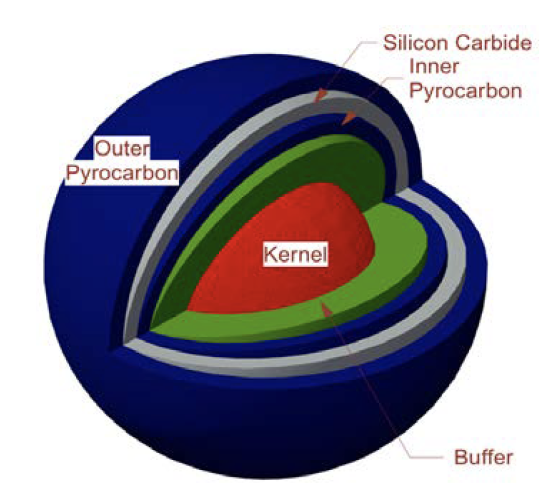
\includegraphics[width=0.35\linewidth]{ahtr-triso.png} 
    \caption{\acrlong{AHTR}'s TRISO particle schematic \cite{noauthor_fluoride_nodate}.}
    \label{fig:ahtr-triso}
\end{figure}

Burnable poisons and control rods for reactivity control are also included in 
some configurations of the \gls{AHTR}. 
The burnable poisons consist of europium oxide, $Eu_2O_3$ and have a discrete
or integral (dispersed) option. 
In the discrete option, small spherical $Eu_2O_3$ particles are stacked axially 
at 5 locations in each fuel plank, as shown in Figure \ref{fig:discrete-poison}. 
\begin{figure}[]
    \centering
    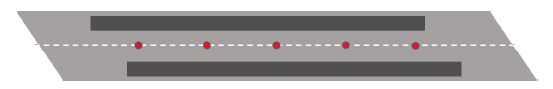
\includegraphics[width=0.6\linewidth]{discrete-poison.png} 
    \caption{Placement of axial stacks of burnable poisons in the \acrlong{AHTR} 
    \cite{noauthor_fluoride_nodate}.}
    \label{fig:discrete-poison}
\end{figure}
In the integral option, $Eu_2O_3$ is homogenously mixed with the fuel plank 
graphite matrix (including the graphite in fuel stripes matrix and the 
graphite in the plank ends indented to structural sides, but excluding the 
graphite in spacers and graphite in TRISO particles). 
Each control rod is uniformly composed of \gls{MHC} and is inserted into the 
Y-shaped control rod slot and displaces the \gls{FLiBe} that occupies the slot
(Figure \ref{fig:ahtr-fuel-assembly}). 

\section{Benchmark Specifications: Phase I}
\label{sec:phase1}
Phase I of the \gls{FHR} benchmark consists of a steady-state 2D model 
(phase I-A) and depletion (phase I-B) of one \gls{FHR} fuel assembly. 
For a single fuel assembly, the internal 120-degree rotational symmetry is 
represented by periodic boundary conditions, as seen in Figure \ref{fig:bc}. 
\begin{figure}[]
    \centering
    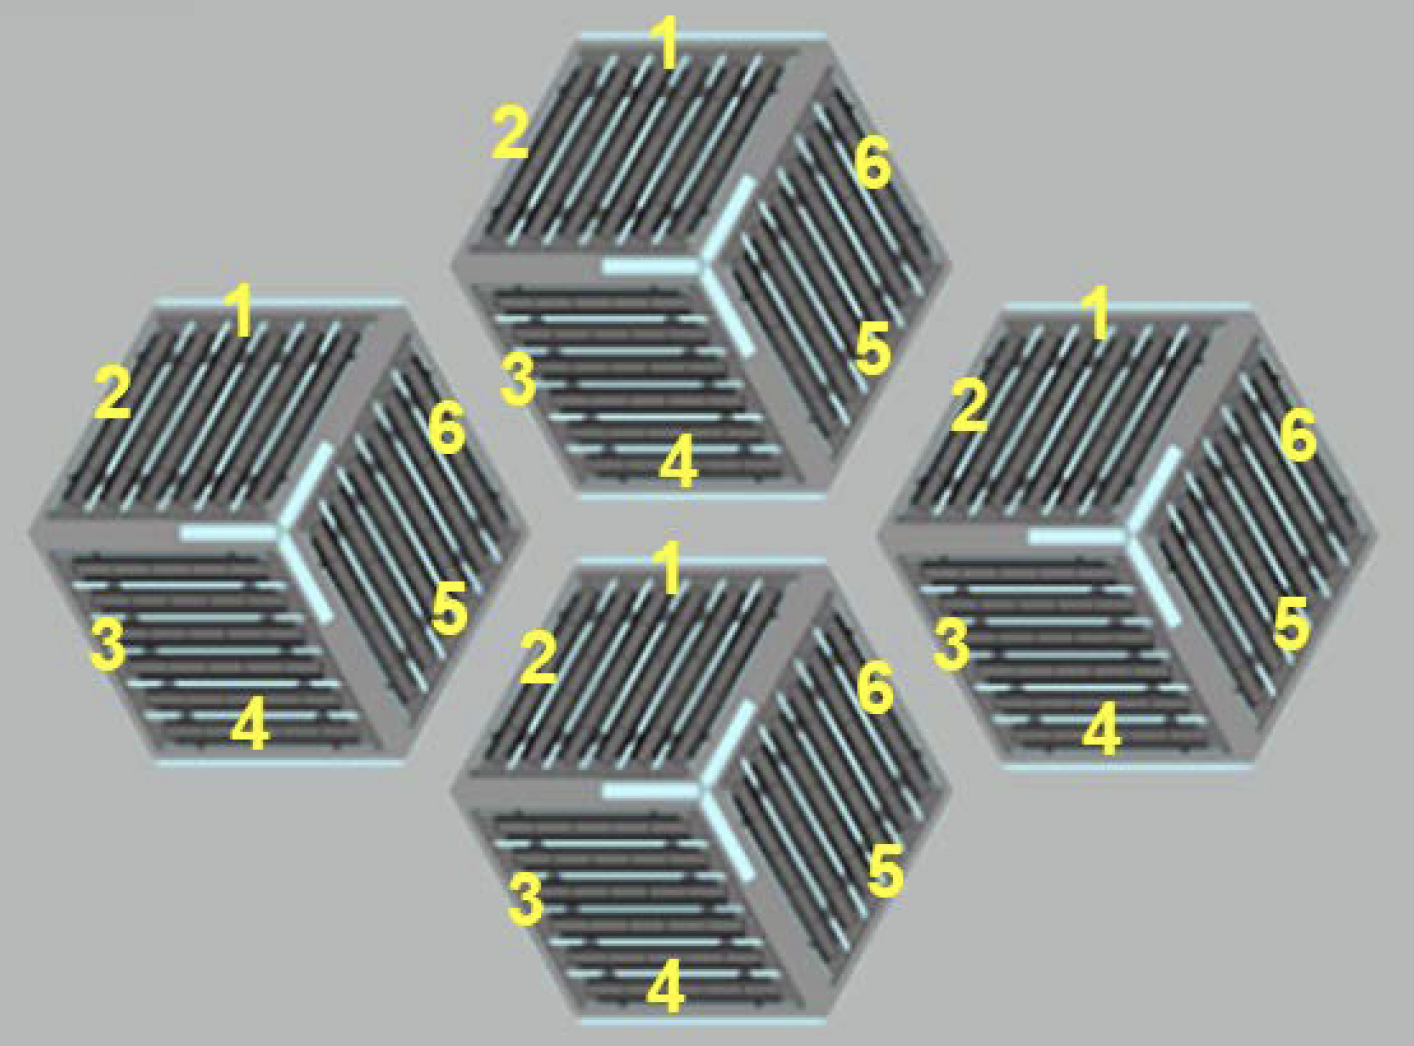
\includegraphics[width=0.5\linewidth]{bc.png} 
    \caption{Visualization of periodic boundary conditions for a single fuel 
    assembly \cite{noauthor_fluoride_nodate}.}
    \label{fig:bc}
\end{figure}
The benchmark required the following results for phases I-A and I-B:
\begin{enumerate}[label=(\alph*)]
    \item Effective multiplication factor 
    \item Reactivity coefficients ($\beta_{eff}$, fuel Doppler coefficient, FLiBe 
    temperature coefficient, graphite temperature coefficient)
    \item Tabulated fission source distribution by 1/5-th fuel stripe. 
    \item Neutron flux averaged over the whole model tabulated in three coarse energy groups. 
    \item Neutron flux distribution in three coarse energy groups
    \item Fuel assembly averaged neutron spectrum
\end{enumerate}

Next, we will report the equations we used to calculate the required results 
listed above. 

\subsubsection{Reactivity Coefficients (b)}
Effective delayed neutron fraction ($\beta_{eff}$) is the fraction of delayed 
neutrons in the core at creation at thermal energies. 
We assumed 1 energy group and 6 delayed groups for $\beta_{eff}$: 
\begin{align}
    \beta_{eff} = \sum_k \beta_k
\end{align}

Reactivity coefficient is the change in reactivity of the material per degree 
change in the material's temperature. 
We calculated each reactivity coefficient and its corresponding uncertainty 
with these equations: 
\begin{align}
    \frac{\Delta \rho}{\Delta T} &= 
    \frac{\rho_{T_{high}}-\rho_{T_{low}}}{T_{high}-T_{low}} [\frac{pcm}{K}] \\
    \delta \frac{\Delta \rho}{\Delta T} &= 
    \frac{\sqrt{\delta (\rho_{T_{high}})^2+(\delta \rho_{T_{low}})^2}}{T_{high}-T_{low}} [\frac{pcm}{K}] 
\end{align}

\subsubsection{Fission Source Distribution / Fission Density (c)}
We calculated \gls{FD} with OpenMC's \texttt{fission} score (f) for a region 
divided by the average \texttt{fission} score of all the regions:
\begin{align}
    FD_i &=  \frac{f_i}{f_{ave}} \\
    \intertext{where}
    f_i &= \mbox{Total fission reaction rate [reactions/src]} \nonumber \\
    f_{ave} &= \mbox{average of all $f_i$ [reactions/src]} \nonumber
\end{align}
The uncertainty calculations for $f_{ave}$ and $FD_i$: 
\begin{align}
    \delta f_{ave} &= \frac{1}{N}\sqrt{\sum_i^Nf_i^2} \\
    \delta FD_i &= |FD_i| \sqrt{(\frac{\delta f_i}{f_i})^2+(\frac{\delta f_{ave}}{f_{ave}})^2} \\
    \intertext{where}
    N &= \mbox{No. of fission score values} \nonumber
\end{align}

\subsubsection{Neutron Flux (d, e, f)}
OpenMC's \texttt{flux} score are in [$\frac{n * cm}{src}$] units. 
For the benchmark, we converted flux to [$\frac{n}{cm^2s}$] units
using the following equations:  

\begin{align}
    \Phi_c &= \frac{N* \Phi_o}{V} \\
    N &= \frac{P*\nu}{Q*k} \\
    \intertext{where}
    \Phi_c &= \mbox{Converted Flux [$\frac{neutrons}{cm^2s}$]} \nonumber \\ 
    \Phi_o &= \mbox{Original Flux [$\frac{neutrons* cm}{src}$]} \nonumber \\
    N &= \mbox{Normalization factor [$\frac{src}{s}$]} \nonumber \\
    V &= \mbox{Volume of fuel assembly [$cm^3$]} \nonumber \\
    P &= \mbox{Power [$\frac{J}{s}$]} \nonumber \\
    \nu &= \mbox{$\frac{\nu_f}{f}$ [$\frac{neutrons}{fission}$]} \nonumber \\
    Q &= \mbox{Energy produced per fission [$\frac{J}{fission}$]} = \mbox{$3.2044*10^{-11}$ J per $U_{235}$ fission} \nonumber \\
    k &= \mbox{$k_{eff}$ [$\frac{neutrons}{src}$]} \nonumber 
\end{align}
Flux standard deviation: 
\begin{align}
    \delta \Phi_c = \Phi_c * 
    \sqrt{(\frac{\delta \Phi_o}{\Phi_o})^2+ (\frac{\delta \nu_f}{\nu_f})^2 
    + (\frac{\delta k}{k})^2 + (\frac{\delta f}{f})^2}
\end{align}
We calculated reactor power based on the given reference specific power 
($P_{sp}$) of 200 $\frac{W}{gU}$. 
\begin{align}
    P &= P_{sp} * V_F * \rho_F * \frac{wt\%_{U}}{100} \\
    \intertext{where}
    V_F &= \mbox{volume of fuel [$cm^3$]} = \frac{4}{3} \pi r_f^3 * N_{total} \nonumber \\
    r_f &= \mbox{radius of fuel kernel} \nonumber\\
    N_{total} &= \mbox{total no. of TRISO particles in fuel assembly} \nonumber\\ 
    &= 101 * 210 * 4 * 2 * 6 * 3 \nonumber\\
    \rho_F &= \mbox{density of fuel [$g/cc$]} \nonumber \\
    wt\%_{U} &= \frac{at\%_{U235} * AM_{U235} + at\%_{U238} * AM_{U238}}{\sum (at\%_i * AM_i)} * 100 \nonumber\\
    AM &= \mbox{atomic mass} \nonumber
\end{align}

\subsection{Benchmark Specifications: Phase I-A}
For phase I-A, the benchmark specifies that each participant must produce a 
steady-state 2D model of one fresh fuel assembly for 9 cases
and report the required results listed in Section \ref{sec:phase1}.  
Table \ref{tab:phase1a-cases} describes each case. 
\begin{table}[H]
    \centering
    \onehalfspacing
    \caption{Description of cases in Phase I-A of the \gls{FHR} benchmark \cite{noauthor_fluoride_nodate}.}
	\label{tab:phase1a-cases}
    \footnotesize
    \begin{tabular}{p{0.05\textwidth}|p{0.9\textwidth}}
    \hline 
    \textbf{Case} & \textbf{Description} \\
    \hline
    1A & Reference case. Hot full power (HFP), with temperatures of 1110K for 
    fuel kernel and 948K for coolant and all other materials (including TRISO 
    particle layers other than fuel kernel). Nominal (cold) dimensions, 
    9 wt\% enrichment, no \gls{BP}, \glspl{CR} out.\\
    \hline
    2AH & \Gls{HZP} with uniform temperature of 948 K, 
    otherwise same as CASE 1A. Comparison with CASE 1A provides HZP-to-HFP power 
    defect.\\
    \hline 
    2AC & \Gls{CZP}. Same as CASE 2AH, but with uniform temperature 
    of 773 K. Comparison with CASE 2AH provides isothermal temperature coefficient.\\
    \hline
    3A & \gls{CR} inserted, otherwise same as CASE 1A. \\
    \hline
    4A & Discrete europia \gls{BP}, otherwise same as CASE 1A.\\
    \hline
    4AR & Discrete europia \gls{BP} and \gls{CR} inserted, otherwise same as 
    CASE 1A. \\
    \hline
    5A & Integral (dispersed) europia \gls{BP}, otherwise same as CASE 1A. \\
    \hline
    6A & Increased \gls{HM} loading (4 to 8 layers of \gls{TRISO}) decreased C/HM 
    (from about 400 to about 200) and decreased specific power to 100 W/gU, 
    otherwise same as CASE 1A.\\
    \hline 
    7A & Fuel enrichment 19.75 wt\%, otherwise same as CASE 1A.\\
    \hline 
    \end{tabular}
\end{table}

\subsection{Benchmark Specifications: Phase I-B}
For phase I-B, the benchmark specifies that each participant must produce 
depletion results for three cases: 1B, 4B, and 7B. 
These are the same as cases 1A, 4A, and 7A, but with depletion steps added and
the critical spectrum assumption. 
The benchmark assumes that depletion occurs only in the fuel and \glspl{BP}. 
Table \ref{tab:phase1b} outlines the results required by the benchmark at specific 
depletion burnup steps for all three cases. 

\begin{table}
    \centering
    \caption{\gls{FHR} benchmark Phase I-B required results at specific burnup 
    steps \cite{noauthor_fluoride_nodate}.}
    \label{tab:phase1b}
    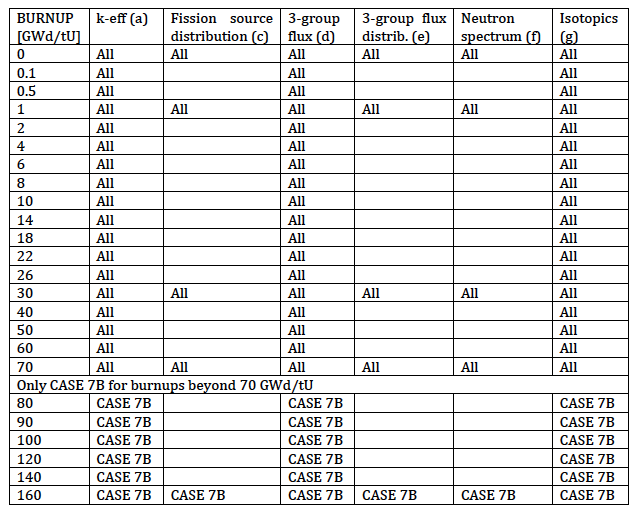
\includegraphics[width=0.8\linewidth]{phase1b.png}
  \end{table}

\section{Results}
Several organizations participated in the benchmark with various Monte Carlo
and Deterministic neutronics codes, such as Serpent \cite{leppanen_serpent_2014}, 
OpenMC \cite{romano_openmc_2013}, and WIMS \cite{lindley_current_2017}. 
We participated in the benchmark with the OpenMC Monte Carlo code 
\cite{romano_openmc_2013} and the ENDF/B-VII.1 material library 
\cite{chadwick_endf/b-vii.1_2011}.
The \texttt{fhr-benchmark} Github repository contains all the results submitted 
by \gls{UIUC} for the \gls{FHR} benchmark \cite{chee_arfcfhr-benchmark_2021}. 
The benchmark used a phased blind approach; thus, participants were asked to 
submit phase I-A and I-B results without knowledge of other submissions. 
Petrovic et al. \cite{petrovic_preliminary_2021} describes the preliminary 
results of the benchmark results across several institutions and concludes 
that the overall observed agreement is satisfactory. 
However, notable differences are identified in specific cases suggesting the 
need for further in-depth analysis of those cases. 
In the subsequent sections, we will share the results obtained by \gls{UIUC}.  

\subsection{Results: Phase I-A}
Petrovic et al. \cite{petrovic_preliminary_2021} compared the effective 
multiplication factor for all participants and phase I-A cases in the \gls{FHR} 
benchmark. 
They reported that the standard deviation between participants for each case 
was in the 231 to 514 pcm range, acceptable and notably close given a blind 
benchmark.
This assures us that our phase I-A results are acceptable and in agreement 
with other benchmark participants. 
Next, we will present our results for phase I-A and describe and explain the 
observed trends.

Table \ref{tab:phase1a-cases} reports phase I-A results for effective multiplication 
factor and reactivity coefficients. 
We ran the simulations on \gls{UIUC}'s BlueWaters supercomputer \cite{ncsa_about_2017}
with 64 XE nodes, which each have 32 cores. 
To reduce the statistical uncertainty of keff to $\sim$10pcm, we ran each simulation 
with 500 active cycles, 100 inactive cycles, and 200000 neutrons. 
Each simulation took \gls{WCT} ranging from 2 to 5 hours. 
\begin{table}[H]
    \centering
    \onehalfspacing
    \caption{\gls{FHR} Benchmark UIUC's phase I-A results \cite{chee_arfcfhr-benchmark_2021}.}
	\label{tab:phase1a-results}
    \footnotesize
    \begin{tabular}{cp{2.7cm}cccccc}
    \hline
    \textbf{Case} & \textbf{Summary} & \textbf{WCT [hr]} & \textbf{$k_{eff}$} & 
    \textbf{$\beta_{eff}$}* & 
    \textbf{Fuel} $\frac{\Delta \rho}{\Delta T}$ & 
    \textbf{FliBe} $\frac{\Delta \rho}{\Delta T}$ & 
    \textbf{Graphite} $\frac{\Delta \rho}{\Delta T}$\\
    \hline 
    1A & Reference &2.82&1.39389$\pm$0.00010 & 0.006534 & -2.24$\pm$0.15 & -0.15$\pm$0.15 & -0.68$\pm$0.15\\
    2AH & \gls{HZP} &2.82&1.40395$\pm$0.00010 & 0.006534 & -3.14$\pm$0.15 & -0.20$\pm$0.14 & -0.85$\pm$0.14\\
    2AC & \gls{CZP} &2.75&1.41891$\pm$0.00010 & 0.006534 & -3.36$\pm$0.14 & -0.11$\pm$0.14 & 0.07$\pm$0.14\\
    3A & \gls{CR} &2.49&1.03147$\pm$0.00011 & 0.006534 & -4.03$\pm$0.28 & -0.83$\pm$0.27 & -3.18$\pm$0.29\\
    4A & Discrete \gls{BP} &5.08&1.09766$\pm$0.00010 & 0.006542 & -4.06$\pm$0.24 & -1.55$\pm$0.23 & -6.51$\pm$0.24\\
    4AR & Discrete \gls{BP} + \gls{CR} &4.59&0.84158$\pm$0.00010 & 0.006553 & -5.60$\pm$0.49 & -1.78$\pm$0.46 & -10.44$\pm$0.47\\
    5A & Dispersed \gls{BP} &2.33&0.79837$\pm$0.00009 & 0.006556 & -5.09$\pm$0.40 & -4.87$\pm$0.40 & -22.99$\pm$0.38\\
    6A & Increased \gls{HM} &3.52&1.26294$\pm$0.00011 & 0.006556 & -4.46$\pm$0.19 & 0.16$\pm$0.20 & -0.39$\pm$0.20\\
    7A & 19.75\% Enriched &2.21&1.50526$\pm$0.00010 & 0.006530 & -2.49$\pm$0.13 & -0.12$\pm$0.12 & -0.62$\pm$0.12\\
    \hline
    \multicolumn{5}{l}{* All $\beta_{eff}$ values have an uncertainty of 0.000001.} 
    \end{tabular}
\end{table}

Cases 2AH and 2AC are at zero power, meaning that the fuel assembly is exactly 
critical but not producing any energy. 
For both cases, keff is higher than the reference case 1A, which we attribute to 
lower fuel temperatures; at higher fuel temperatures, doppler broadening occurs 
resulting in more neutron capture, thus, lowering keff. 
As expected, keff is lower for cases 3A, 4AR, and 5A than reference case 
1A since those cases introduced burnable poisons and control rods to the fuel 
assembly. 
Also, as expected, keff is higher for case 7A than reference case 1A since 
the fuel has a higher enrichment. 
However, case 6A deviated from expectations with a lower keff despite an increase 
in \gls{HM} loading. 
This unexpected behavior is due to reduced moderation and worsened fuel 
utilization brought about by self-shielding, demonstrating increase in 
fuel packing fraction does not always correspond with an increased keff. 

$\beta_{eff}$ increased by 10-20pcm for cases 4A, 4AR, 5A, and 6A, compared to
reference case 1A, due to the introduction of control rods and poisons, which 
shifts the average neutron velocity to higher values resulting in decreased
thermal fission and increased fast fission\cite{torabi_neutronic_2018}.
Table \ref{tab:phase1a-results} reports that most of the temperature coefficients 
are negative, exemplifying the \gls{AHTR}'s passive safety behavior. 
Negative reactivity feedback results in a self-regulating reactor; if the reactor's 
power rises, resulting in temperature increase, the negative reactivity will, 
in turn, reduce power. 

Figure \ref{fig:phase1a-c} shows the fission source distribution by 
$1/5^{th}$ fuel stripe for cases 1A and 3A. 
\begin{figure}[]
    \centering
    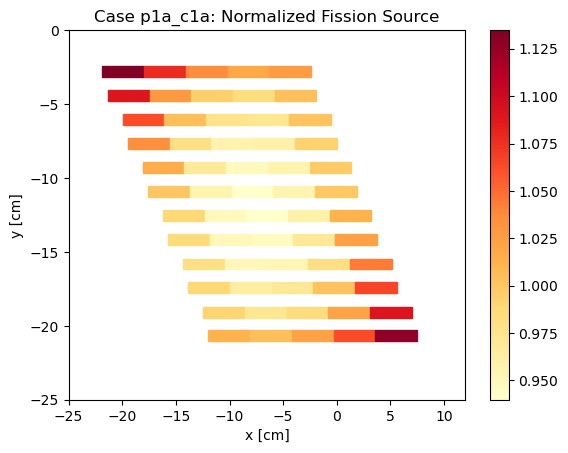
\includegraphics[width=0.49\linewidth]{p1a_c1a_c.png} 
    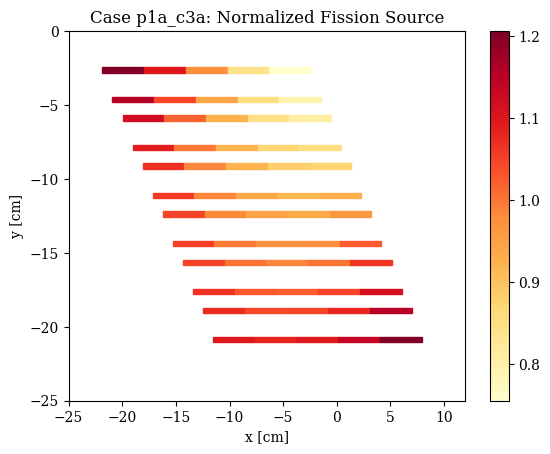
\includegraphics[width=0.49\linewidth]{p1a_c3a_c.png} 
    \caption{Fission Source Distribution per $1/5^{th}$ fuel stripe for \gls{FHR} 
    Benchmark's phase I-A Case 1A (left) and Case 3A (right).}
    \label{fig:phase1a-c}
\end{figure}
Case 4AR has a similar fission source distribution as case 3A since both 
cases have control rod insertion. 
All other cases have similar fission source distributions to case 1A. 
For case 1A, intuitively, we would assume that the highest fission source would 
occur in the center of the diamond fuel segment; however, the opposite is true. 
Power peaking occurs on exterior stripes and is minimum on the interior stripes.
Gentry et al. \cite{gentry_development_2016} reported similar power peaking 
phenomena towards the lattice cell's exterior closest to the Y-shaped carbon 
support structure where the thermal flux is most elevated, and the complement 
to the peaking is found in the interiors of the lattice tri-sections. 
This fission source distribution is caused by diminished resonance escape 
probability in the interior due to the higher relative fuel-to-carbon volume 
ratio. 
This diminished fission source in the interior stripes phenomena is exaggerated 
in cases 6A and 7A since there is a higher fuel-to-carbon ratio.
For case 3A that has an inserted control rod, the fission source is lower in 
the $1/5^{th}$ stripes closer to the control rod.  

Figure \ref{fig:phase1a-d} shows the average neutron flux in the fuel assembly in 
three coarse energy groups. 
\begin{figure}[]
    \centering
    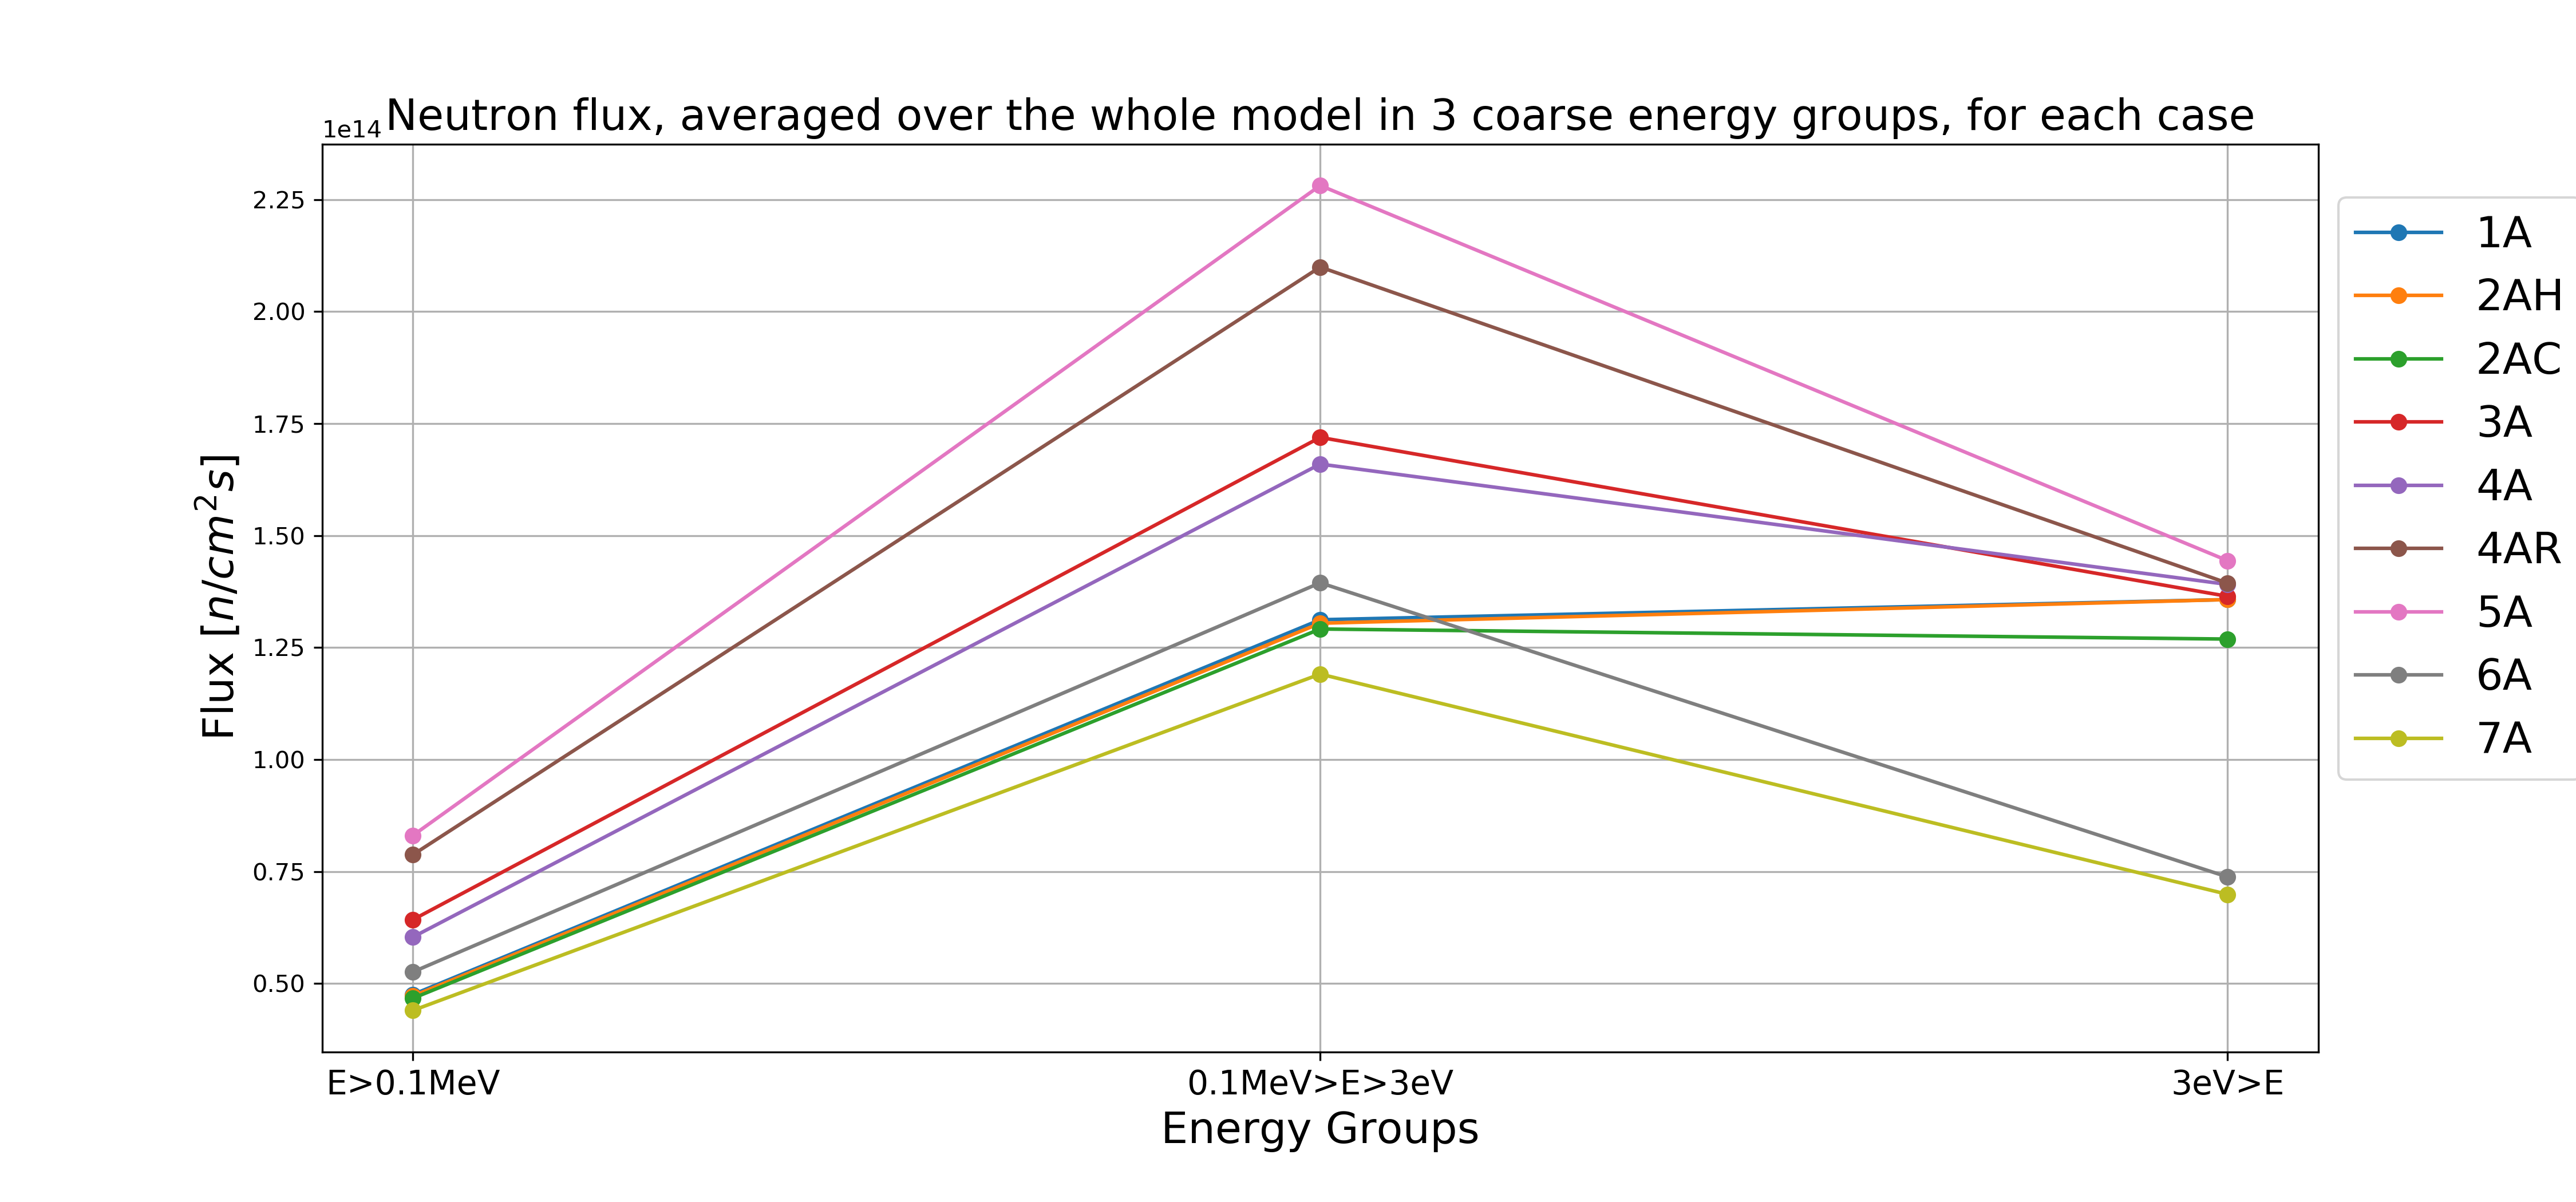
\includegraphics[width=\linewidth]{phase1a-d-flux.png} 
    \caption{Neutron Flux, averaged over the whole model, tabulated in three coarse 
    energy groups for each phase I-A case. }
    \label{fig:phase1a-d}
\end{figure}
Most of the cases have the most flux in the intermediate group, followed by 
the thermal group, and the least flux in the fast group.    
Figure \ref{fig:phase1a-e} shows the neutron flux distribution for case 1A, 
3A, and 6A for three coarse energy groups. 
\begin{figure}[]
    \centering
    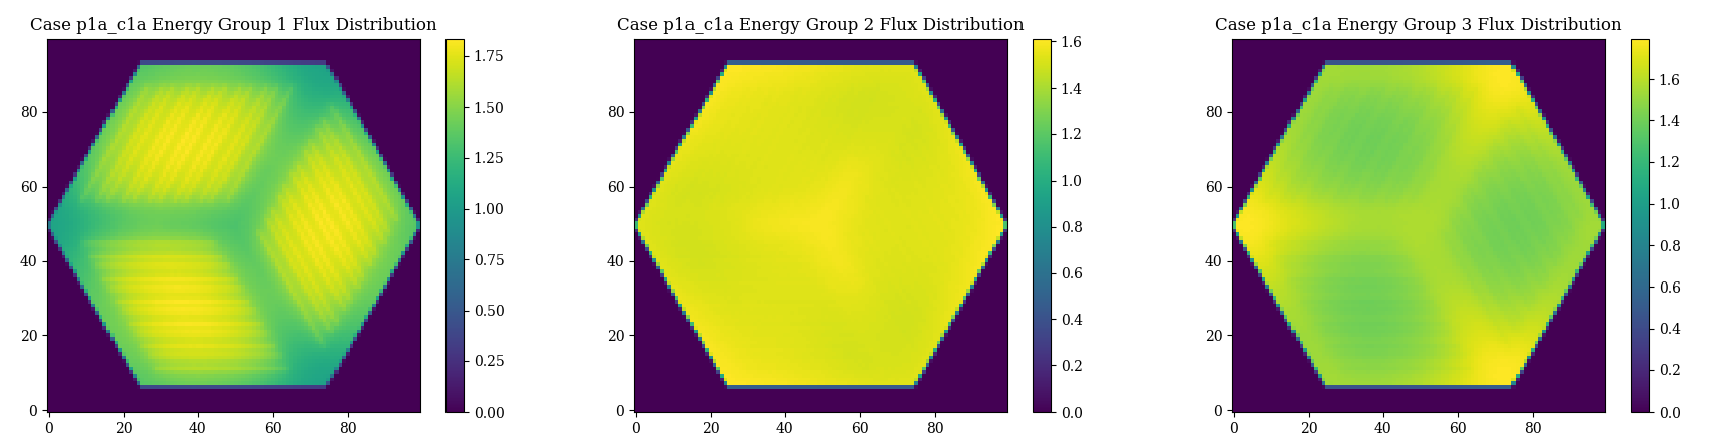
\includegraphics[width=0.9\linewidth]{phase1a-e-c1a.png} 
    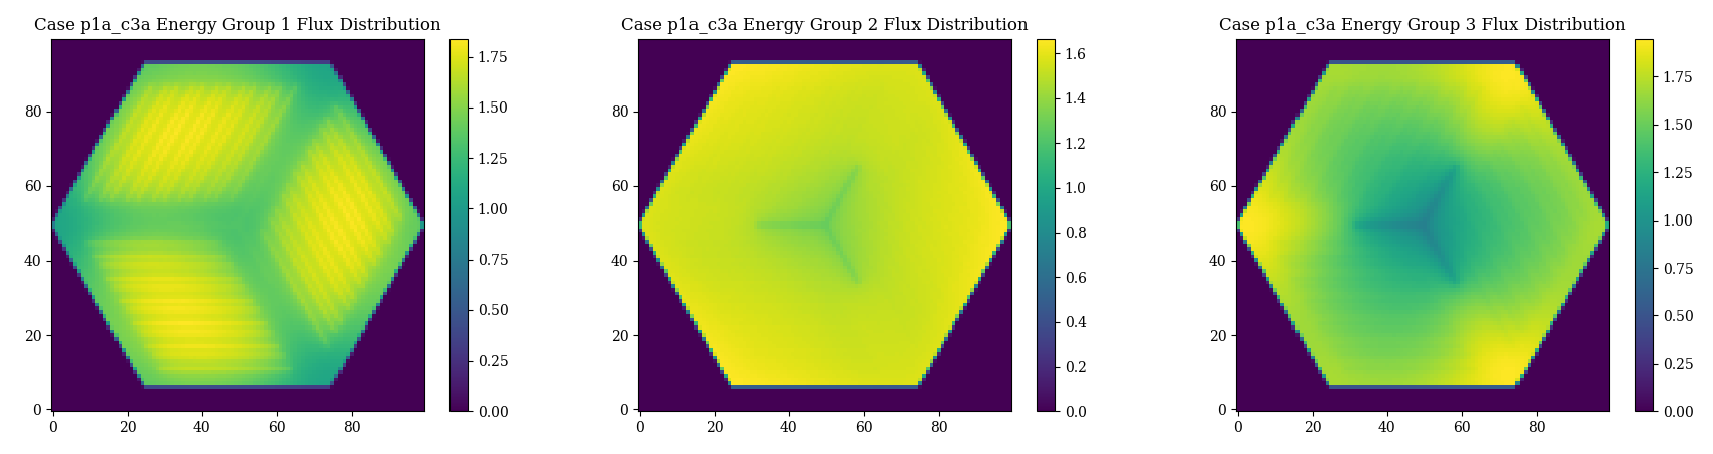
\includegraphics[width=0.9\linewidth]{phase1a-e-c3a.png} 
    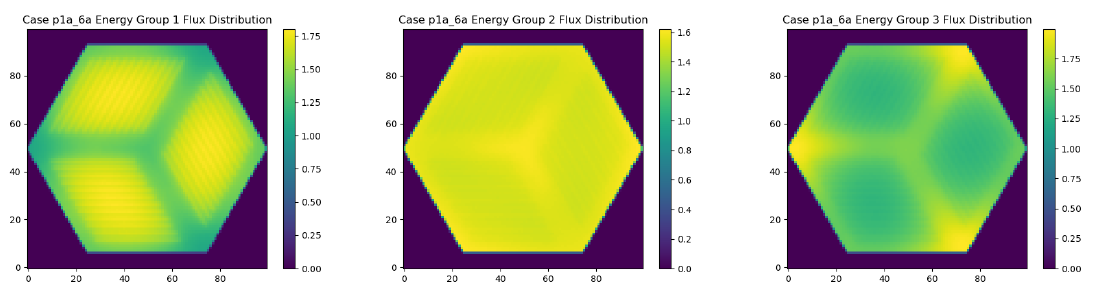
\includegraphics[width=0.9\linewidth]{phase1a-e-c6a.png} 
    \caption{Neutron Flux distribution in 100 by 100 mesh for three coarse 
    energy groups: case 1A (above), case 3A (middle), case 6A (below) }
    \label{fig:phase1a-e}
\end{figure}
For all three cases, fast-flux peaks in the diamond-shaped sectors containing 
the fuel stripes, whereas thermal flux peaks outside of the diamond-shaped 
sectors; this is attributed to fission occurring at thermal energies in the 
fuel stripe area. 
For case 3A, the thermal and intermediate neutron flux is depressed in the fuel 
assembly's control rod region.  
Case 6A has increased \gls{HM}; thus, we see that fast-flux peaking and the 
thermal flux dip in the fuel stripe area is more pronounced than case 1A.
Figure \ref{fig:phase1a-f} shows the neutron spectrum for cases 1A and 6A. 
\begin{figure}[]
    \centering
    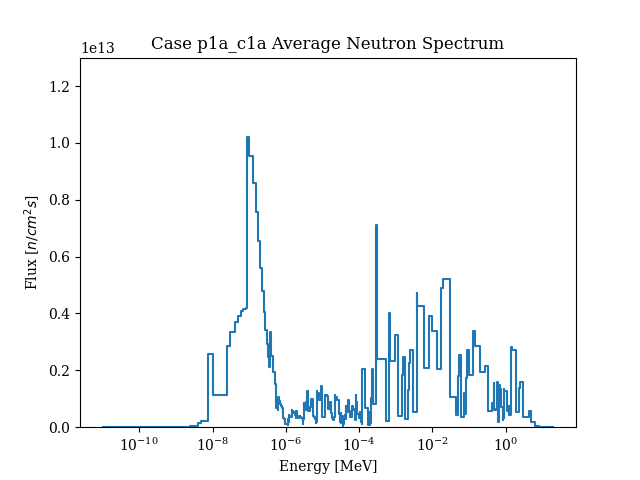
\includegraphics[width=0.49\linewidth]{p1a_c1a_f.png} 
    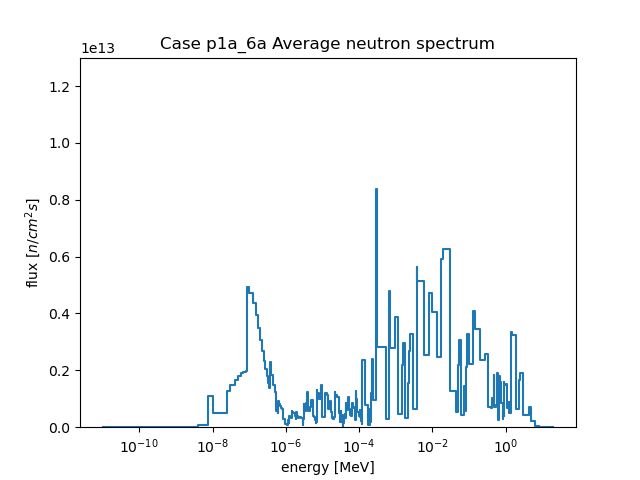
\includegraphics[width=0.49\linewidth]{p1a_c6a_f.png} 
    \caption{Neutron Spectrum for \gls{FHR} Benchmark's phase I-A Case 1A 
    (left) and Case 6A (right).}
    \label{fig:phase1a-f}
\end{figure}
Case 7A has a similar neutron spectrum as case 6A since both cases have 
higher fuel content. 
All other cases have a similar neutron spectrum to case 1A.
The neutron spectrum is faster for case 6a and case 7a due to more heavy metal 
loading and higher enrichment.  

\subsection{Results: Phase I-B}


\section{Summary}
% more enrichment / more HM does not mean higher keff, there is shielding 
% effects, thus, this leads us to believe that the phenomena is not as expected. 

This chapter described the \gls{FHR} benchmark specifications, \gls{AHTR} design,
and the phase I results obtained so far by the UIUC team. 
The benchmark results highlight the \gls{AHTR}'s passive safety behavior with 
negative temperature coefficients. 
Unanticipated results such as a lower keff for the \gls{AHTR} configuration with 
higher \gls{HM} loading gave insight into how increased fuel packing does not always 
correspond with increased keff due to self-shielding.
These results hint at the possibility of minimizing fuel required by optimizing 
for inhomogeneous fuel distributions within the core. 
This will be further explored in the next chapters. 

